%This article is written for students who gonna to speedrun IMO problems with not so good base(for example: the author)
\documentclass{Math_Note}

\title{IMO2024 Solutions}
\author{Buce-Ithon}
\newdateformat{mydate}{\twodigit{\THEDAY}{ }\shortmonthname[\THEMONTH], \THEYEAR}
\date{\today}

\begin{document}

%Title page
\maketitle

%Content
\newpage
\tableofcontents
\newpage

%Problem 1
\section*{Problem 1}
\begin{prb}
    Determine all real numbers $\alpha$ such that, for every positive integer $n$, the integer
    \begin{equation}
        \lfloor\alpha\rfloor + \lfloor 2\alpha \rfloor + \cdots + \lfloor n\alpha \rfloor
    \end{equation}
    is a multiple of n.
    (Note that $\lfloor\alpha\rfloor$ denotes the greatest integer less than or equal to $z$. For 
    instance, $-\lfloor\pi\rfloor=-4$, $\lfloor2\rfloor=\lfloor2.9\rfloor=2$)
\end{prb}

\begin{sol}
As the 1st question of this IMO, it is not so hard to solve it. Let's analyze this problem from a beginner's perspective.
\newline\newline
Look at this formula: $\lfloor\alpha\rfloor + \lfloor 2 \alpha \rfloor + \cdots + \lfloor n\alpha \rfloor$, it rounds each 
term down and adds them together. 

\marginpar{\textcolor{green}{idea}} 
\textcolor{blue}{So a simple idea is: split every term into its integer and fractional parts and observe what happens.} \textcolor{lightblue}{(It's easy to think.)}

\textcolor{blue}{Other idea: Actually you can also find that the formula is similar with arithmetic sequence sum formula, which is 
for summing integers of the same interval. Then discuss the case where $\alpha$ is an integer(as above), and the other case 
where it's not an integer, so all real numbers are included. And you could get same process and result.)}
\newline\newline
\marginpar{\textcolor{green}{solution}}
So, let's split $\alpha$ as $\alpha = [\alpha]+\left\{\alpha\right\}$, the $[\alpha]$ represents the integer part of $\alpha$ and 
$\left\{\alpha\right\}$ represents its fractional part.

\begin{equation}
    \begin{split}
        let\quad S_{n} &= \lfloor\alpha\rfloor + \lfloor2\alpha\rfloor + \cdots + \lfloor n\alpha \rfloor \\
        &= \left(\left[\alpha\right]+\left[2\alpha\right]+\cdots+\left[n\alpha\right]\right) 
           + \left(\left\{\alpha\right\}+\left\{2\alpha\right\}+\cdots+\left\{n\alpha\right\}\right) \\
        &= \left(1+2+\cdots+n\right)\left[\alpha\right] + \left(\left\{\alpha\right\}+\left\{2\alpha\right\}+\cdots+\left\{n\alpha\right\}\right) \\
        &= \frac{n\left(1+n\right)}{2}\left[\alpha\right] + \left(\left\{\alpha\right\}+\left\{2\alpha\right\}+\cdots+\left\{n\alpha\right\}\right) \\
    \end{split}
\end{equation}

For this part $\frac{n\left(1+n\right)}{2}\left[\alpha\right]$:

1. If $\left[\alpha\right]$ is an odd number, then $n\nmid\frac{n\left(1+n\right)}{2}\left[\alpha\right]$ when $n$ is an even number.

2. If $\left[\alpha\right]$ is an even number, then $n\mid\frac{n\left(1+n\right)}{2}\left[\alpha\right]$ for all positive integer $n$.

For rest part $\left\{\alpha\right\}+\left\{2\alpha\right\}+\cdots+\left\{n\alpha\right\}$:

As we all know $\left\{\alpha\right\}\in\left(-1,0\right)\cup\left(0,1\right)$, then 

1. $\forall\alpha\in\left(-1,0\right)$, $\exists$ a positive numner $n$ s.t. $\left(n-1\right)\left\{\alpha\right\}>-1>\left(n\right)\left\{\alpha\right\}$ 
then $\left\{\alpha\right\}+\left\{2\alpha\right\}+\cdots+\left\{n\alpha\right\}=n-1$, and $n\nmid\left(n-1\right)$.

2. Similarly,$\forall\alpha\in\left(0,1\right)$, $\exists$ a positive numner $n$ s.t. $\left(n-1\right)\left\{\alpha\right\}<1<\left(n\right)\left\{\alpha\right\}$
then $\left\{\alpha\right\}+\left\{2\alpha\right\}+\cdots+\left\{n\alpha\right\}=1$, and $n\nmid 1 \forall n\geq2$.
\newline\newline
\marginpar{\textcolor{green}{conclusion}}
Thus, there is the unique station holds for all $n$, that is $\alpha$ is even ($\alpha=2k, k\in\mathrm{Z}$).
\end{sol}

%Problem 2
\section*{Problem 2}
\begin{prb}
    Determine all pairs $\left(a,b\right)$ of positive integers for which there exist positive integer $g$ and $N$ such that 
    \begin{equation}
        gcd\left(a^{n}+b,b^{n}+a\right) = g
    \end{equation}
    holds for all integers $n\geq N$. (Note that $gcd(x,y)$ denotes the greatest common divisor of integer $x$ and $y$)
\end{prb}
\begin{sol}
The next problem seems more difficult. But, in fact, when we try some simple cases and pay attention to the exponential $n$, we can 
associate it with Euler's theorem and then construct the solution.
\newline\newline
\marginpar{\textcolor{red}{motivation}}
Let's first try some easy and special cases as following: 

\textcolor{blue}{
1. $\left(a,b\right)=\left(1,1\right)$, then $gcd\left(a,b\right)=gcd\left(1^{n}+1,1^{n}+1\right)=2, \forall n\in\mathrm{Z^{+}}$. \\ 
2. $\left(a,b\right)=\left(k,k\right)$, then $gcd\left(a,b\right)=gcd\left(k^{n}+k,k^{n}+k\right)=k^{n}+k$, is not a fixed number as $n$ changes. \\
3. $\left(a,b\right)=\left(1,k\right)$, then $gcd\left(a,b\right)=gcd\left(1+k,k^{n}+1\right)$, as $k$ is an odd number, $1+k\mid1+k^{n}$, 
then $gcd\left(a,b\right)=1+k$; as $k$ is an odd number, then $k^{n}+1\equiv k\left(k^{n-1}+1\right)-\left(k+1\right)+2\equiv 2 \left(mod(1+k)\right)$. \\
4. $\left(a,b\right)=\left(2,3\right)$, then $gcd\left(a,b\right)=gcd\left(2^{n}+3,2+3^{n}\right)$ \\
you'll find: \\
\begin{table}[h!]
    \begin{center}
    \textcolor{blue}{
    \begin{tabular}{|c|c|c|c|c|c|c|}
        \hline
        n & $2^{n}+3$ & $3^{n}+2$ & L mod 5 & R mod 5 & L mod 7 & R mod 7 \\
        \hline
        1 & $5$ & $5$ & $0$ & $0$ & $5$ & $5$ \\
        \hline
        2 & $7$ & $11$ & $2$ & $1$ & $0$ & $4$ \\
        \hline
        3 & $11$ & $29$ & $1$ & $4$ & $4$ & $1$ \\
        \hline
        4 & $19$ & $83$ & $4$ & $3$ & $5$ & $6$ \\
        \hline
        5 & $35$ & $245$ & $0$ & $0$ & $0$ & $0$ \\
        \hline
        6 & $67$ & $731$ & $2$ & $1$ & $4$ & $3$ \\
        \hline
        7 & $131$ & $2189$ & $1$ & $4$ & $5$ & $5$ \\
        \hline
    \end{tabular}}
    \end{center}
\end{table}
\\
It's periodic.\\
Although it not correct answer. But it indicates us an approach to find something that divides $gcd\left(a^{n}+b,b^{n}+a\right)$ regularly but 
doesn't divide the $gcd$ the other terms, and this will eliminate some $\left(a,b\right)$ as valid solution.\\
As observing the list above again, we could find $gcd\left(2,3,5\right)=1$ and $gcd\left(2,3,7\right)=1$, moreover for some $n\geq N\in\mathbb{Z}^{+}$, 
$5\vert 2^{n}+3, 5\vert 3^{n}+2$ and $7\vert 2^{n}+3, 7\vert 3^{n}+2$.\\
(So far, we can guess $\left(1,1\right)$ is the unique solution and prove it in this direction.)
}
\newline
\marginpar{\textcolor{red}{idea}}
\textcolor{lightblue}{
Think about it, if $gcd\left(a^{n}+b,b^{n}+a\right) = g$ holds for all integers $n \geq N$, then the $gcd$ $g$ must have some factors which are coprime 
with $a^{n}+b$ and $b^{n}+a$.\\ 
And vice versa, if a number $q$ satisfies $gcd\left(q,a^{n}+b\right)=gcd\left(q,b^{n}+a\right)=1$ and $q\vert a^{n}+b, q\vert b^{n}+a$ for some $n\geq N$
(for infinitly many numbers $n$), then $q\vert gcd\left(a^{n}+b,b^{n}+a\right)$.\\
This $q$ will help us figure out this question, if we could find some uniqueness or counterexample about $q$.\\
}
\newline
\marginpar{\textcolor{red}{solution}}
If(Let) $g=gcd\left(a^{n}+b,a+b^{n}\right)$ for some $n\geq N$ exists, then 
\begin{equation}
    g\vert a^{n}+b,\quad g\vert a+b^{n}
\end{equation}
For some $N\in\mathbb{Z}^{+} (exists), n\geq N$, the number $g$ has a factor, we set it as $q$, then
\begin{equation}
    q\vert g \Longrightarrow q\vert a^{n}+b,\quad q\vert a+b^{n}
\end{equation}
\textcolor{blue}{
(Ok, we can use this $q$ to prove $\left(a,b\right)$ must be $\left(1,1\right)$, no other else solutions!)
}
Let's analyze it: 
\begin{equation}
    \begin{split}
        q &\vert a^{n}+b,\quad q\vert a+b^{n}\\
        q &\vert a^{n+1}+b,\quad q\vert a+b^{n+1}
    \end{split}
\end{equation}
then we get 
\begin{equation}
    \begin{cases}
        q\vert a^{n+1}-a^{n} \Longrightarrow q\vert a^{n}\left(a-1\right)\\
        q\vert b^{n+1}-b^{n} \longrightarrow q\vert b^{n}\left(b-1\right)
    \end{cases}
\end{equation}
\textcolor{blue}{
(Here, if $gcd\left(q,a\right)>1$, then let $q=gcd\left(q,a\right)\cdot q^{'}$, we have 
$gcd\left(q^{'},a\right)=1$ and $q^{'}\vert a^{n}\left(a-1\right)$. Similiar with $q$ and $b$.)\\
}
So set \underline{$gcd\left(q,a\right)=1$ and $gcd\left(q,b\right)=1$}, then \underline{$q\vert a-1, q\vert b-1$ for some $n\geq N$}.\\
With our intuition, we can construct $q=ab+1$. \\
\marginpar{\textcolor{green}{tip}}
\textcolor{blue}{
(Some people may confused with it, let me try to explain: 
$1^{\circ}.$ you can find the fact from the motivation we ever tried before, $gcd(2,3,5)=gcd(2,3,7)=1$, 
$2^{\circ}.$ it's a seemly common fact that $gcd\left(ab,ab+1\right)=1 \left(gcd\left(n,n+1\right)=1\right)$)\\
}
Let's first prove our assumptions, which are marked by underline: 
\begin{enumerate}
    \item It's easy to verify $gcd\left(ab+1,a\right)=gcd\left(ab+1,b\right)=1$. (Because $gcd\left(ab+1,ab\right)=1$. Proof by contradiction.)
    \item We ganna to prove $q\vert a-1,\quad q\vert b-1$, \\
    which is equal to $ab+1\vert a^{n}+b,\quad ab+1\vert a+b^{n}$ since $gcd\left(q,a\right)=gcd\left(q,b\right)=1$. \\
    Observing that $ab+1=a^{-1}\left(a^{2}b+a\right)=a\left(b+a^{-1}\right)$, \\
    then taking with $a^{n}+b$(pay attention to the index position), it inspires us the Fermat's Theorem (exactly Euler-Fermat's Theorem). \\
    Hense let $n=k\cdot\phi(ab+1)-1$ (for some $k\in\mathbb{Z}^{+}$), then 
    \begin{equation}
        \begin{split}
            a\left(a^{n}+b\right) \equiv a\cdot a^{k\cdot\phi(ab+1)-1}+ab &\equiv a\left(a^{-1}+b\right) \left(mod\ ab+1\right) \\
            and\quad a\left(a^{-1}+b\right) &\equiv 0 \left(mod\ ab+1\right)
        \end{split}
    \end{equation}
    Then $ab+1\vert a\left(a^{n}+b\right)$, also since $gcd\left(ab+1,a\right)=1$, then for some $n=k\cdot\phi(ab+1)-1$, $ab+1\vert a^{n}+b$. 
    Similarly, we have $ab+1\vert a+b^{n}$. \\
    Then $q\vert a-1$ and $q\vert b-1$ for some $n\geq N=k_{0}\cdot\phi(ab+1)-1$ is proved.
\end{enumerate}
Finally, if $g\vert a^{n}+b, g\vert b+a^{n}$, we must have for some $n\geq N$, $ab+1\vert a-1, ab+1\vert b-1$.\\
And since 
\begin{equation}
    \begin{cases}
        ab+1 \leq a-1 \\
        ab+1 \leq b-1 
    \end{cases}
    and\ 
    \begin{cases}
        ab+1 \geq a-1 \\
        ab+1 \geq b-1
    \end{cases}
\end{equation}
\textcolor{blue}{
(the left inequations is obtained by the property of congruence, the right hand is easy to notice)\\
}
thus 
\begin{equation}
    \begin{cases}
        ab+1 = a-1 \\
        ab+1 = b-1 
    \end{cases}
    \left(no\ way\right)\ or\ 
    \begin{cases}
        a=1 \\
        b=1 
    \end{cases}
\end{equation}
The problem is solved.
\end{sol}

%Problem 3
\newpage
\section*{Problem 3}
\begin{prb}
    Let $a_{1}, a_{2}, a_{3}, \cdots$ be an infinite sequence of positive integers, and let $N$ be a positive integer. Suppose that, for each $n>N$, 
    $a_{n}$ is equal to the numbers of times $a_{n-1}$ appears in the list $a_{1}, a_{2}, \cdots, a_{n-1}$.

    Prove that at least one of the sequence $a_{1}, a_{3}, a_{5}, \cdots$ and $a_{2}, a_{4}, a_{6}, \cdots$ is eventually periodic. (An infinite sequence 
    $b_{1}, b_{2}, b_{3}, \cdots$ is eventually periodic if there exists positive integers $p$ and $N$, s.t. $\forall m>N, b_{m}=b_{m+p}$.)
\end{prb}
\begin{sol}
This is not only the hardest peoblem in day 1, but also the most insane in this IMO with the unique combination. \\
Actually after several tries, I can not figure it out or even find some useful clue. So I post and explain the general solution for learner to study deeply. \\
\newline
\marginpar{\textcolor{green}{explore}}
\textcolor{blue}{
To solve the combination problems, it seems to be likely to solving the functional equation problems: 
try, explore and find the features. \\
}
\newline
Lemma 1. (1) Some integers appear infinitely many times. $\longleftrightarrow$ (2) $\{a_{n}\}$ is unbounded. \\
\textcolor{lightblue}{
Proof:  
$1^{\circ}.$ If (1) is not true, then $\forall n_{1}\in\mathbb{Z}^{+}, \exists n_{2}\in\mathbb{Z}^{+}$, s.t. $max\{a_{1},\cdots,a_{n_{1}}\}\leq a_{n_{2}}$, i.e. 
$\{a_{n}\}$ is unbounded. Then there are totally infinitely many $1$ after this number, which is a contradiction. (There must be infinitely many increasing numbers.) \\
$2^{\circ}.$ If (2) is not true, then there are some numbers appearing infinitely many times. With the definition of $a_{n}$, there is the contradiction. \\
}
Lemma 2. Let $M=max\{a_{1},a_{2},\cdots,a_{N}\}$, for every integer $x>M$ appears at most $M$ times. \\
\textcolor{lightblue}{
Proof:  
If it's not true, consider the first time that any $x>M$ appears for the $M^{th}$ time. Up to this point, each appearance of $x$ is preceded by an integer which has appeared $x>M$ times. 
So there must have been at least $M$ numbers that have already appeared at least $M$ times before $x$ does, which is a contradiction. \\
}
\begin{figure}[H]
    \centering
    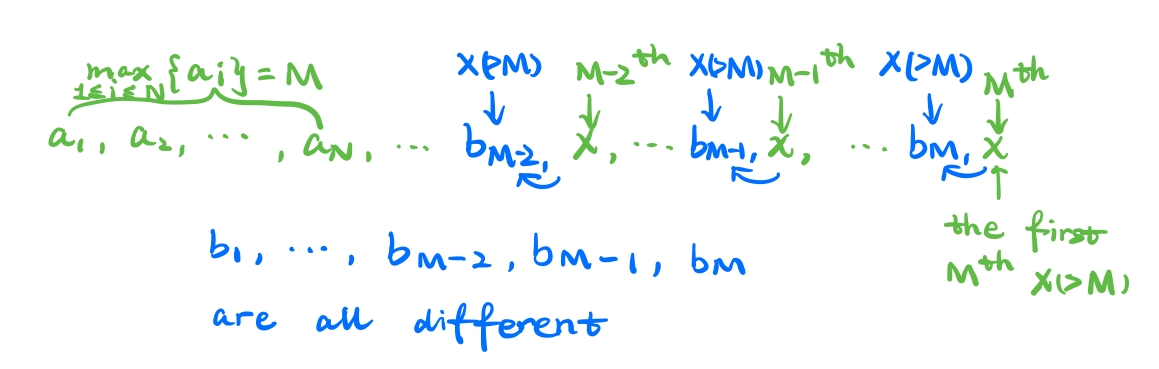
\includegraphics[scale=0.25]{"./Figures/Q3F1.png"}
    \caption{Lemma 2-proof}
\end{figure}
Lemma 2-1. There are only finitely many numbers that appear infinitely many times. \\
\marginpar{\textcolor{green}{idea}}
Development: 
\textcolor{lightblue}{Set $k$ is the largest of these finitely many numbers. There are infinitely many different numbers $j$ before every $k$ having appeared $k^{th}$ times (after $a_{N}$). 
And here more important point is: the former $j$ has appeared $k-1^{th}$ times, then the $k-1$ appears infinitely many times.} And so on, $1, 2,\cdots, k$ all appear infinitely many times. \\
Since $k+1$ doesn't appear infinitely often, there must only be finitely many numbers which appear more than $k$ times. \textcolor{lightblue}{(The reason is similiar to the above.)} Let the largest such number be $l\geq k$. \\
From here on, we call an integer $x$ big if $x>l$, medium if $l\geq x>k$ and small if $x\leq k$. \\
To summarise, each small number appears infinitely many times in the sequence, while each big number appears at most $k$ times in the sequence. \\
\begin{figure}[H]
    \centering
    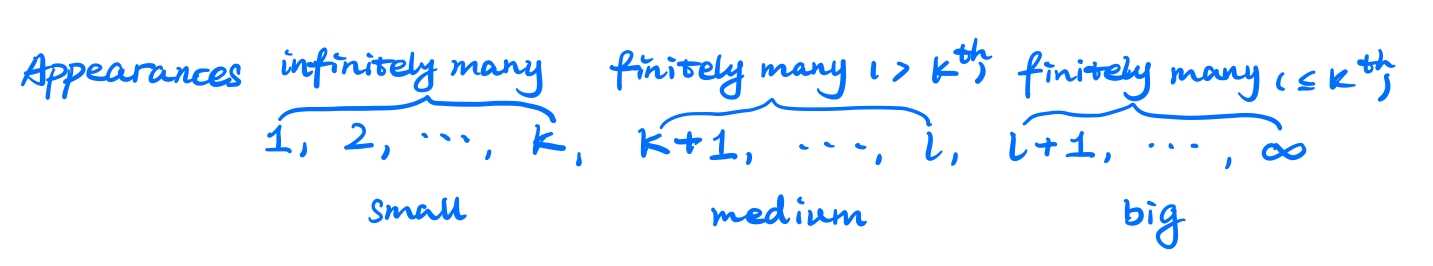
\includegraphics[scale=0.25]{"./Figures/Q3F2.png"}
    \caption{Lemma 2-1-development}
\end{figure}
\marginpar{\textcolor{green}{method}}
Process: 
Choose a large enough $N^{'}>N$ s.t. $a_{N^{'}}$ is small, and in $a_{1},\cdots,a_{N^{'}}$: 
\begin{itemize}
    \item every medium number has already made all of its appearances
    \item every small number has made more than $max\{l,N\}$ appearances
\end{itemize}
Since every small has appeared more than $l$ times before $a_{N^{'}}$, past this point each small number must be followed by a big number (greater than $l$). Also, by definition, 
each big number appears at most $k$ times, so it must be followed by a small number. Hence the sequence alternates between big and small number after $a_{N^{'}}$. \\
Lemma 3. Let $g$ be a big number that appeared after $a_{N^{'}}$. If $g$ is followed by the small number $h$, then $h$ equals the amount of small numbers which have appeared at least $g$ times before that point. \\
\textcolor{lightblue}{
Proof: 
By the definition of $N^{'}$, the small number immediately preceding $g$ has appeared more than $max\{l,N\}$ times, so $g>max\{l,N\}$. And since $g>N$, the $g^{th}$ appearance of every small nummber 
must occur after $a_{N}$ and hence is followed by $g$. \\
Since there are $k$ small numbers and $g$ appears at most $k$ times, $g$ must appear exactly $k$ times, always following a small number after $a_{N}$. Hence on the $h^{th}$ appearance of $g$, exactly $h$ small numbers 
have appeared at least $g$ times before that point. \\
}
Denote by $a_{\left[i,j\right]}$ the subsequence $a_{i}, a_{i+1},\cdots, a_{j}$. \\
Lemma 4. Suppose that $i$ and $j$ satisfy the following conditions: \\
(a) $j>i>N^{'}+2$ \\
(b) $a_{i}$ is small and $a_{i}=a_{j}$ \\
(c) no small value appears more than once in $a_{\left[i,j-1\right]}$ \\
Then $a_{i-2}$ is equal to some small number in $a_{\left[i,j-1\right]}$. \\
\textcolor{lightblue}{
Proof: 
Let $\mathcal{I}$ be the set of small number that appear at least $a_{i-1}$ times in $a_{\left[1,i-1\right]}$. By Lemma 3, $a_{i}=\vert\mathcal{I}\vert$. Similarly, let $\mathcal{J}$ be the set of small numbers 
that appear at least $a_{j-1}$ times $a_{\left[1,j-1\right]}$. Then by Lemma 1, $a_{j}=\vert\mathcal{J}\vert$ and hence by (b), $\vert\mathcal{I}\vert=\vert\mathcal{J}\vert$. Also by definition, $a_{i-2}\in\mathcal{I}$ 
and $a_{j-2}\in\mathcal{J}$. \\
Suppose the small number $a_{j-2}$ is not in $\mathcal{I}$. This means $a_{j-2}$ has appeared less than $a_{i-1}$ times in $a_{\left[1,i-1\right]}$. By (c), $a_{j-2}$ has appeared at most $a_{i-1}$ times in 
$a_{\left[1,j-1\right]}$, hence $a_{j-1}\leq a_{i-1}$. Combining with $a_{\left[1,i-1\right]}\subset a_{\left[1,j-1\right]}$, this implies $\mathcal{I}\subset\mathcal{J}$. But since $a_{j-2}\in\mathcal{J}\backslash\mathcal{I}$, 
this contradicts $\vert\mathcal{I}\vert=\vert\mathcal{J}\vert$. So $a_{j-2}\in\mathcal{I}$, which means it has appeared at least $a_{i-1}$ times in $a_{\left[1,i-1\right]}$ and one more time in $a_{\left[i,j-1\right]}$. So, 
$a_{\left[j-1\right]}>a_{\left[i-1\right]}$. \\
By (c), any small number appearing at least $a_{j-1}$ times in $a_{\left[1,j-1\right]}$ has also appeared $a_{j-1}-1\geq a_{i-1}$ times in $a_{\left[1,i-1\right]}$. So $\mathcal{J}\subset\mathcal{I}$ and hence $\mathcal{I}=\mathcal{J}$. 
Therefore, $a_{i-2}\in\mathcal{J}$, so it must appear at least $a_{j-1}-a_{i-1}=1$ more time in $a_{\left[i,j-1\right]}$. \\
}
\newline
\marginpar{\textcolor{softcyan}{Genius}}
For each small number $a_{n}$ with $n>N^{'}+2$, let $p_{n}$ be the smallest number such that $a_{n+p_{n}}=a{i}$ is also small for some $i$ with $n\leq i<n+p_{n}$. In other words, $a_{n+p_{n}}=a_{i}$ is the first small number to 
occur twice after $a_{n-1}$. If $i>n$, Lemma 4 (with $j=n+p_{n}$) implies that $a_{i-2}$ appears again before $a_{n+p_{n}}$, contradicting the minimality of $p_{n}$. So $i=n$. \\
Lemma 2 also implies that $p_{n}\geq p_{n-2}$. So $p_{n}, p_{n+2}, p_{n+4}, \cdots$ is a nondecreasing sequence bounded above by $2k$ (as there are only $k$ small numbers). Therefore, $p_{n}, p_{n+2}, p_{n+4}, \cdots$ is eventually 
constant and the subsequence of small numbers is eventually periodic with period at most $k$. \\
\newline
Problem solved. 
\end{sol}

%Problem 4
\newpage
\section*{Problem 4}
\begin{prb}
    Let $\Delta ABC$ be a triangle with $AB<AC<BC$. Let the incentre and incircle of triangle $ABC$ be $I$ and $\omega$. Let $X$ be the point on line $BC$ different from $C$ 
    s.t. the line through $X$ parallel to $AC$ is tangent to $\omega$. Similarly, let $Y$ be the point on line $BC$ different from $B$ such that the line through $Y$ parallel 
    to $AB$ is tangent to $\omega$. Let $AI$ intersect the circumcircle of triangle $\Delta ABC$ again at $P \neq A$. Let $K$ and $L$ be the midpoints os $AC$ and $AB$, respectively.

    Prove that $\angle KIL + \angle YPX = 180^{\circ}$. 
\end{prb}
\begin{sol}
As the unique geometry problem in this IMO, it's not so hard a question, even a bit easy and interesting. 

Let's draw the graph of the problem first. 

\begin{figure}[H]
    \centering
    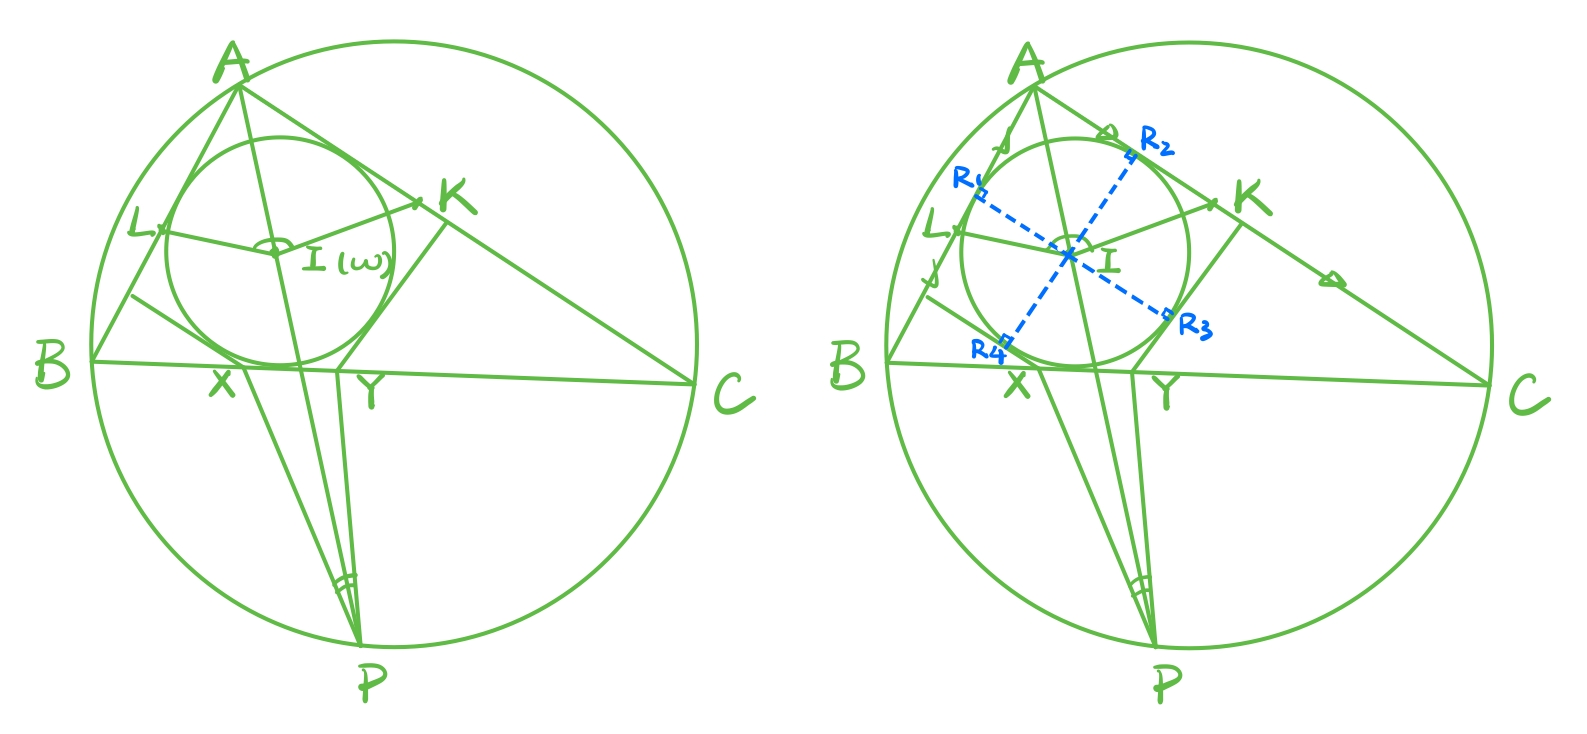
\includegraphics[scale=0.22]{"./Figures/Q4F1.png"}
    \caption{Figure from the problem}
\end{figure}
\marginpar{\textcolor{green}{review}}
\textcolor{blue}{
As you can see, the circle $\omega$(later note $\odot I$) with center $I$ is the incircle of $\Delta ABC$. \\
$L, K$ are the midpoints of $AB, AC$, and $X, Y$ are the intersection point of $BC$ and the lines parallel to $AC, AB$ and tangent to $\odot I$. \\
$P$ is the intersection point of line $AI$ and circumcircle of $\Delta ABC$. }

If we label the intersection points of $\odot I$ and $\Delta ABC$ as $R_{1}, R_{2}, R_{3}, R_{4}$. 

It's not so hard to notice that $R_{1}R_{3} \bot AB, R_{3}Y$ and $R_{2}R_{4} \bot AC, R_{4}Y$. With our junior high school mathematics fundation, $AI$ is the angle bisector of $\angle BAC$. 
Then we can get a lot of equality and parallel relations. 
\newline\newline
\marginpar{\textcolor{green}{point}}
\textcolor{blue}{
So if we extend segments $R_{4}X$ and $R_{3}Y$, their intersection point shoud be in line $AP$. And it will double length segment $AI$. (Actually, the method of doubling $AI$ is similir or 
even same with this idea.)}
\newline\newline
\marginpar{\textcolor{green}{solution}}
As the following figures, we extend $R_{4}X$ and $R_{3}Y$ noting the intersection as point $Z$. 

It's easy to get(properties of angle bisector): $\angle R_{1}AI=\angle R_{2}AI=\angle R_{3}ZI=\angle R_{4}ZI$. 
\begin{figure}[H]
    \centering
    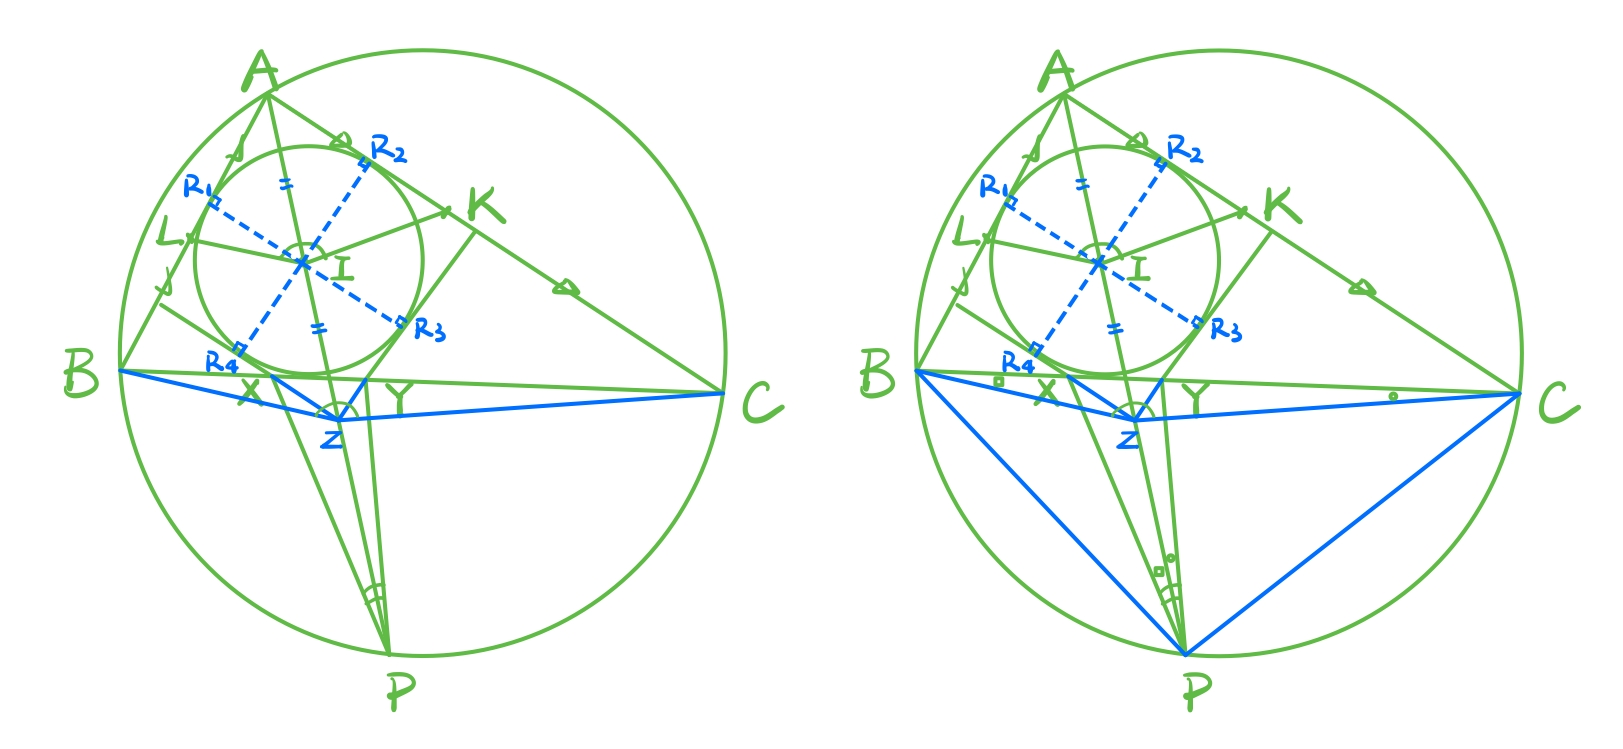
\includegraphics[scale=0.22]{"./Figures/Q4F2.png"}
    \caption{Add guidelines}
\end{figure}
Since $AB \parallel R_{3}Z$ and $R_{1}I=R_{3}I$, then using the simplest proportional relation (or you can use the similarity of triangles), we'll get $AI=IZ$.

(Notation: $\parallel$ means 'parallel to'.)

And as $AL=BL, AK=CK$($L, I, K$ are midpoints of $AB, AZ, AC$), then connecting $BZ$ and $CZ$, we have $BZ \parallel LI, CZ \parallel KI$. 

Then using the simplest similarity relation, $\angle AIL=\angle AZB, \angle AIK=\angle AZC$, then $\angle BZC=\angle LIK$. 

Now, the question is transformed to prove $\angle KIL+\angle XPY=\angle BZC+\angle XPY=180^{\circ}$. 

But in this moment, as our observing, in triangle $\Delta BZC$, $\angle BZC+\angle ZBC+\angle ZCB=180^{\circ}$. 

Can we transform or let $\angle XPY=\angle ZBC+\angle ZCB$ ? No more suspence, certainly we can! 

Let's transform it a bit more: $\left(\angle XPY=\right)\angle XPZ+\angle YPZ=\angle ZBC+\angle ZCB$. 

\marginpar{\textcolor{green}{point2}}
If we connecting $BP, PC$ (for convenience), with our intuition ($\angle XPZ$ and $\angle ZBX(\angle ZBC)$ point to the same chord $XZ$), 
it inspires us to prove $X,Z,P,B$ and $Y,Z,P,C$ are in a circle. 

\begin{figure}[H]
    \centering
    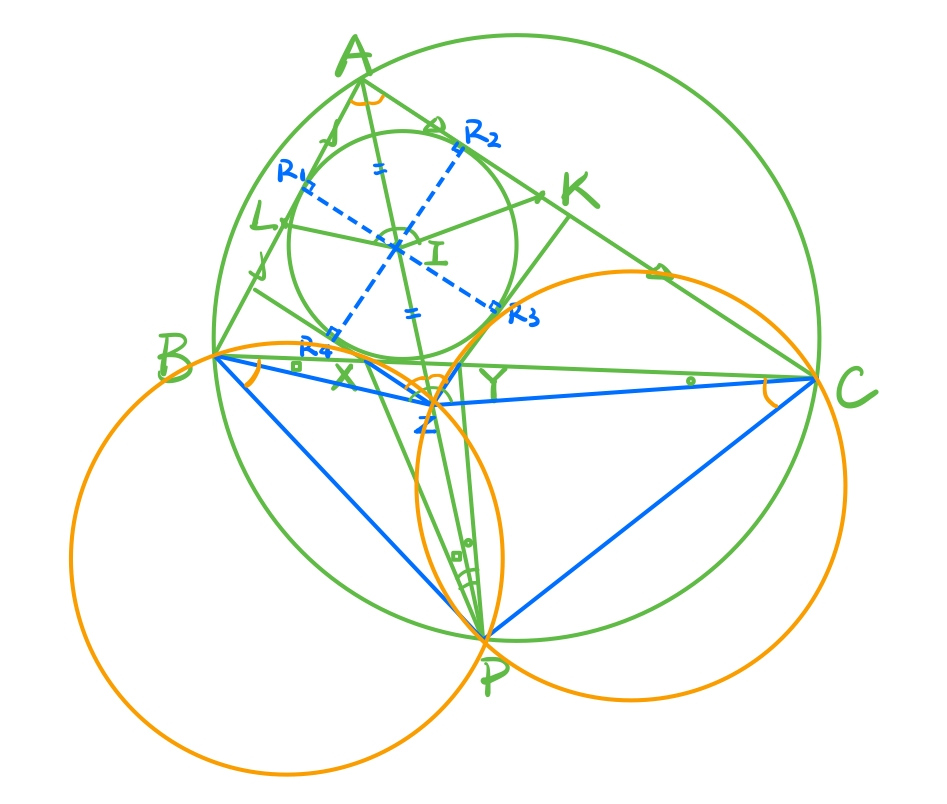
\includegraphics[scale=0.25]{"./Figures/Q4F3.png"}
    \caption{Final run}
\end{figure}

Since in circumcircle of $\Delta ABC$, $\angle PBC$ and $\angle PAC$ point to same chord $PC$, then $\angle PBC=\angle PAC$. 

With the relation we get earlier: $\angle R_{1}AI=\angle R_{2}AI=\angle R_{3}ZI=\angle R_{4}ZI$, 

we have $\angle PBC=\angle XZA$, then $\angle PBX+\angle XZP=180^{circ}=\angle BPZ+\angle BXZ$. 

Then we have $X,Z,P,B$ in a same circle. Similarly, with symetry, $Y,Z,P,C$ is in same circle. 

Since that, $\angle XPZ=\angle ZBX, \angle YPZ=\angle ZCY$. 

Thus,
\begin{equation}
    \begin{split}
        \angle KIL+\angle XPY &= \angle BZC+\left(\angle XPZ+\angle YPZ\right)\\
        &= \angle BZC+\left(\angle ZBC+\angle ZCB\right) \\
        &= 180^{\circ}. 
    \end{split}
\end{equation}

It's proved.

\end{sol}

%Problem 5
\newpage
\section*{Problem 5}
\begin{prb}
    Turbo the snail plays a game on a board with 2024 rows and 2023 columns. There are hidden monsters in 2022 of the cells. Initially, Turbo doesn't know 
    where any of the monsters are, but he knows that there is exactly one monster in each row except the first and last row, and each column contains at most one monster.

    Turbo makes a series of attempts to go from the first row to the last row. On each attempt, he choose to start on any cell in the first row, the repeatedly moves to an 
    adjacent cell sharing a common side. (He is allowed to return to a previously visited cell.) If he reaches a cell with a monster, his attempt ends and he is transported 
    back to the first row to start a new attempt. The monsters don't move, and Turbo remembers wether or not each cell he has visited contains a monster. If he reaches any 
    cell in the last row, his attempt ends and the game is over.

    Determine the minimum value of $n$ for which Turbo has a strategy that guarantees reaching the last row on the $n^{th}$ attempt or earlier, regardless of the locations 
    of the monsters. 
\end{prb}
\begin{sol}
\marginpar{\textcolor{green}{motivation}}
\textcolor{blue}{
It's the most interesting problem in this IMO! \\
So let's think about a simple situation as following: \\
\begin{figure}[H]
    \centering
    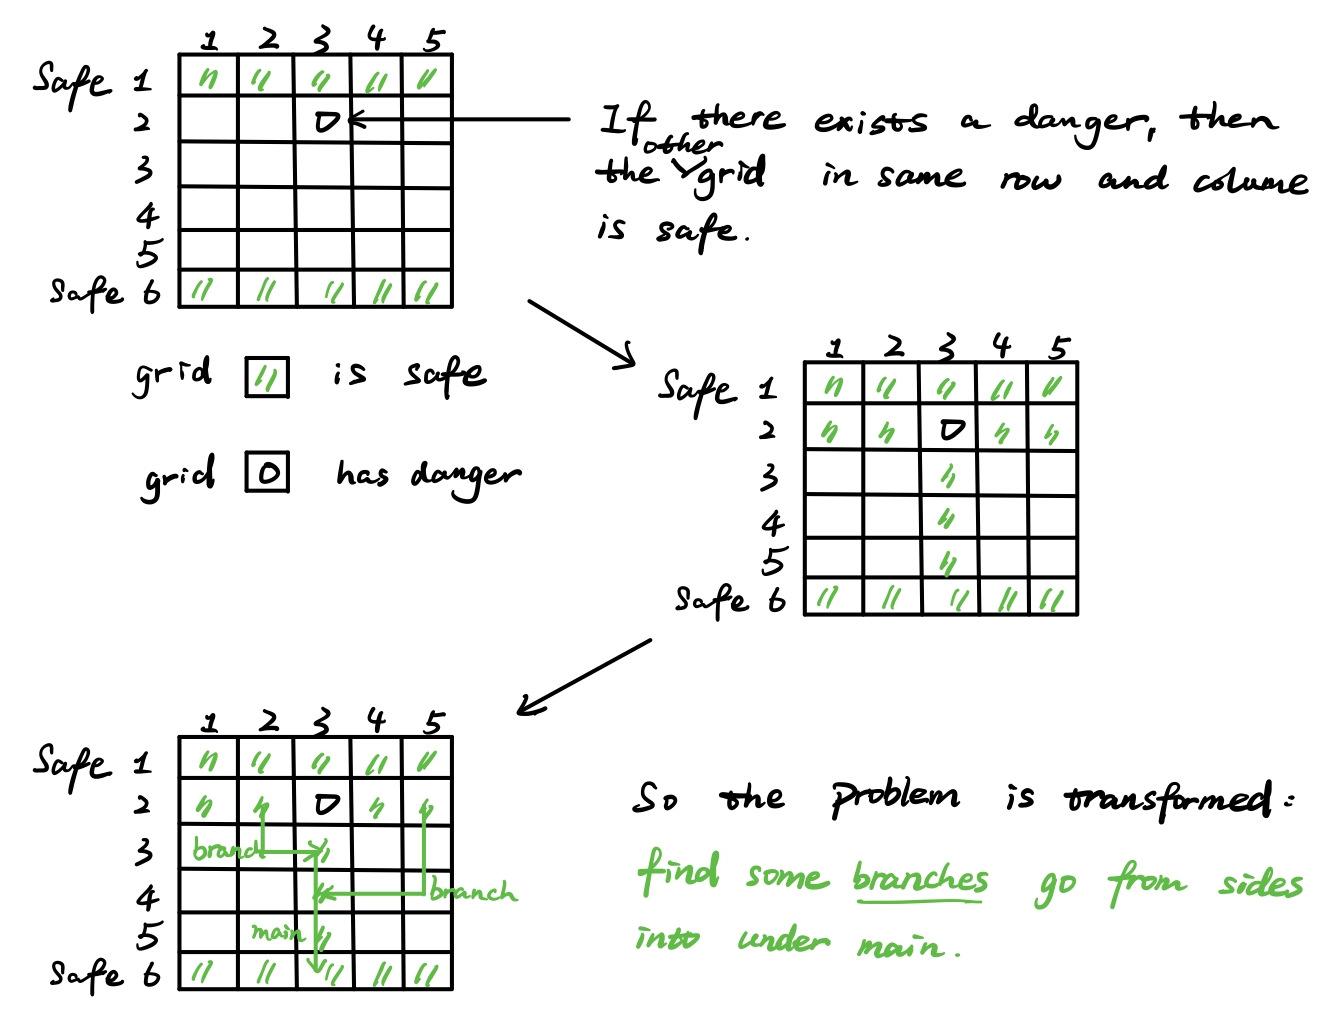
\includegraphics[scale=0.25]{"./Figures/Q5F1.png"}
    \caption{Simple situation-have a try}
\end{figure}
To briefly describe, I simplify the original 2024$\times$2023 table into 6$\times$5 (rows $\times$ column, notation $(x,y)$). \\
The first row $(1,\sim)$ and last row $(6,\sim)$ is safe, and all safe grid is marked by green double-short slash. \\
And according to the problem, in rest grids (from $(2,1)$ to $(5,5)$, 4$\times$5), there are at most $1$ monster (called as 'danger' in figures, marked by black circle). \\
\newline
If we find one monster(danger) in one row, for instance 2nd row $(2,\sim)$, it means the rest grid in same row and column are safe.\\
\newline
Then the all blocks in the next column under this danger are safe, which means moreover, we find a safe passage to the end.\\
And next we just need to find a safe branch into this safe main passage, the Turbo will get it way! \\
}
\newline
\marginpar{\textcolor{green}{solution}}
Ok, let's get our thoughts in order and figure it out! \\
$1^{\circ}.$ \underline{First step}: find the unique danger in 2nd row.
\begin{figure}[H]
    \centering
    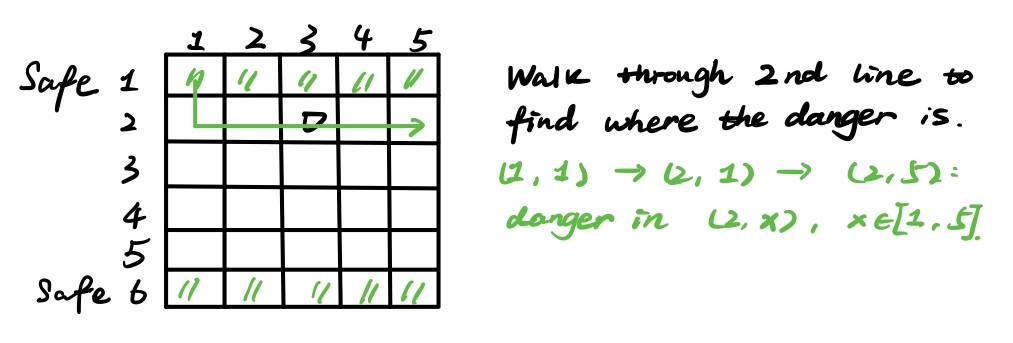
\includegraphics[scale=0.25]{"./Figures/Q5F2.png"}
    \caption{First step}
\end{figure}
Walk through the 2nd row to find where the danger is (for later discussion of classification). The route is: $\left(1,1\right)\rightarrow\left(2,1\right)\rightarrow\left(2,5\right)$.\\
Mark the danger in $(2,y), y\in\left[1,5\right]$. \\
$2^{\circ}.$ \underline{Second step}: find the safe branch to main passage.
It's clear to classify 2 situations to discuss next portion. 
\begin{enumerate}
    \item The danger is in two sides. $y=1$ or $y=5$.
    \begin{figure}[H]
        \centering
        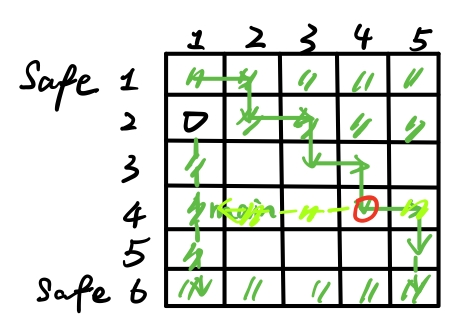
\includegraphics[scale=0.25]{"./Figures/Q5F3_1.png"}
        \caption{Second step-situation 1-side}
    \end{figure}
    A magic strategy is take the step-down route. This is a too simple idea to clasrify, but I can provide a thought for reference. \\
    As you can see, when we find the 2nd-row danger in $(2,1)$ ($(2,5)$ is similiar), the safe grids has been marked with green notation. \\
    So the rest unclear grids form a rectangle, with only one danger in each row. \\
    \marginpar{\textcolor{green}{method}}
    \textcolor{blue}{
    Neither walking horizontally nor walking certically can guarantee that we can find the safe branch in the least number of times, espcially 
    in some special cases (such as all dangers are on the same diagonal). Then we try to go diagonally. \\
    }
    The wonderful point of this method is: once Turbo encounter the danger, the left grids in this row and the grids he walked must be safe. And in 
    above graph, this grids just happen to be connected into a safe branch! (Actually, it's the reason leading me to this method.) \\
    The route is: $(1,1)\rightarrow(1,2)\rightarrow(2,2)\rightarrow(2,3)\rightarrow(3,3)\rightarrow(3,4)\rightarrow(4,4)\rightarrow(4,5)\rightarrow(5,5)\dashrightarrow(5,6)$. 
    \item The danger is in the middle. $y\in\left[2,4\right]$.
    \begin{figure}[H]
        \centering
        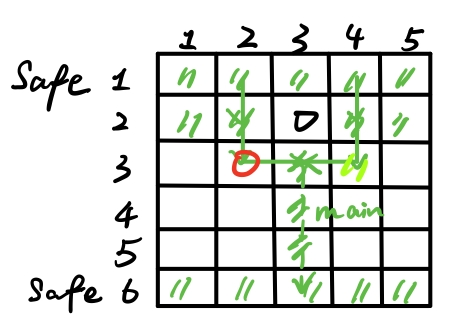
\includegraphics[scale=0.25]{"./Figures/Q5F3_2.png"}
        \caption{Second step-situation 2-middle}
    \end{figure}
    This situation is common and easy. \\
    Because there are at most one danger in every row. Then we just need to find the danger on the next adjacent diagonal line. \\
    Worst situation is entouring a danger and the other is absolutely safe, or they are all safe (it's the best). \\
    The route is (suppose dagher is in $(2,3)$): $(1,2)\rightarrow(2,2)\rightarrow(3,2)\rightarrow(3,3)\rightarrow(6,3)$ or $(1,4)\rightarrow(2,4)\rightarrow(3,4)\rightarrow(3,3)\rightarrow(6,3)$.
\end{enumerate}
Thus, after '2-step verification' Turbo can definitely find the correct and safe route.
\newline\newline
\marginpar{\textcolor{green}{extra}}
\textcolor{lightblue}{
An extra question: The method I introduced in 2nd step 1st situation is easy but may not suit for eavry body. Is there any wonderful way for 2nd step-situation 1-sides or other situation and step to find a safe branch?
}
\end{sol}

%Problem 6
\newpage
\section*{Problem 6}
\begin{prb}
    Let $\mathbb{Q}$ be the set of rational numbers. A function $f: \mathbb{Q}\rightarrow\mathbb{Q}$ is called aquaesulian if the following property holds: for every $x,y\in\mathbb{Q}$, 
    \begin{equation}
        f(x+f(y))=f(x)+y \quad or \quad f(f(x)+y)=x+f(y).
    \end{equation}
    Show that there exists an integer $c$ s.t. for any aquaesulian function $f$ there are at most $c$ different rational numbers of the form $f(r)+f(-r)$ for some rational number $r$, 
    and find the smallest possible value of $c$. 
\end{prb}
\begin{sol}
As the last problem in 65th IMO, it is a typical and beautiful functional equations problem. \\
\marginpar{\textcolor{softcyan}{reflection}}
\textcolor{softcyan}{
Before we starting solving this problem, I gonna to share a little my self feeling or thoughts about this kind of problems: \\
In my eyes, the functional equation is using to describe something either special or abstract with some 'features'. \\
For the questioner, constructing a function often depends on practical problems or personal wild ideas (majority). \\
For those of us who solve the problems, it's not so easy to directly to konw what is it exactly, so we often gonna to find the 'features' of 
the functional equation (now we call it properties of this function) just like finding bugs in playing video games. And it's a funny process. \\
So, for me, the interests is not solving this problem, it's to figure it out: what is it. That's most important! \\
}
\marginpar{\textcolor{softcyan}{attempts}}
1. Reviewing the problem, we could find the functional equations is actually 2 mapping (f) from $x+f(y)$ and $f(x)+y$.\\
\begin{equation}
    \begin{cases}
        x \mapsto f(x) \\
        y \mapsto f(y)
    \end{cases}
    \quad
    x+f(y) \underset{f}{\overset{f}{\rightleftharpoons}} f(x)+y
\end{equation}
2. The most simple try: let $x=y=0$, then $\underline{f(f(0))=f(0)}$. \\
\textcolor{softcyan}{
(If you have some experience, you may try to find if $f(0)=0$, which means more better 'features' or methods. Me too. But don't worry, let's observe it carefully first to find what can we learn.)\\
}
If we ganna to find $f(0)=a, a\in R$, there are 2 strategies: $1^{\circ}$ directly to find $f(0)=a$ from equations (12), $2^{\circ}$ $f(\underline{f(0)})=f(\underline{0}) \Longrightarrow f(0)=0$ (from image to preimage).\\
3. The other common try: let $f(x)=x$, then the 2 mapping in equation (13) are all satisfied. Then $f(x)$ is aquaesulian (special case). \\
For $f(x)=x$, we can easy find $f(r)+f(-r)=r+(-r)=0$, which means there are unique rational numbers (only one) can be expressed as $f(r)+f(-r)$. So we estimate that $\underline{c\geq 1}$. \\
4. Another (maybe not easy) try: let $y=-f(x)$, then 
\begin{equation}
    f(x+f(-f(x)))=0 \quad or \quad f(0)=x+f(-f(x))
\end{equation}
An magic intuition seems to lead us to calculate the value of $f(x)$. \\
5. So this is the 4th try (let's see what kind of mapping $f$ is): \\
let $\underline{f(x)=f(y)}$, then without loss of generality, we have $f(x)+y=f(x+f(y))=f(x+f(x))=f(x)+x$. Then $\underline{x=y}$. It means $f(x)$ is \underline{injective}.\\
6. The 4th try is a very useful feature, because it just corresponds to the 2nd strategy in 2. \\
Combining 2.$2^{\circ}$ and 5, we have $f(f(0))=f(0)$ indicates $\underline{f(0)=0}$. \\
7. Taking 6 with 4, we have $f(x+f(-f(x)))=0=f(0) \quad or \quad 0=f(0)=x+f(-f(x))$. It indicates $x+f(-f(x))=0$, or $\underline{-x=f(-f(x))\ or\ x=f(-f(-x))}$, which means $f(x)$ is \underline{surjective}. \\
\begin{equation}
    x \mapsto f(x), then -f(x) \mapsto -x
\end{equation}
Then $f(x)$ is a \underline{bijection}, and $\underline{f^{-1}(x)=-f(-x)}$. \\
\newline
8. Let's do the last but magic try: 
\begin{equation}
    \begin{split}
        & f^{-1}(x) \mapsto x \mapsto f(x) \\
        & f^{-1}(y) \mapsto y \mapsto f(y)
    \end{split}
\end{equation}
Observing that $f(x)=f(x)+f(-x)-f(-x)=f(x)+f(-x)+f^{-1}(x)$, as before, we have known $c\geq 1$, now we try to test if $c$ can be greater than $2$: \\
\newline
If we set $f(x)+f(-x)=a$ and $f(y)+f(-y)=b$ for some $a\neq b$, then $f(x)=a+f^{-1}(x)$, similiar with $f(y)$. \\
Hense 
\begin{equation}
    \begin{split}
        & f^{-1}(x) \mapsto x \mapsto a+f^{-1}(x) \\
        & f^{-1}(y) \mapsto y \mapsto b+f^{-1}(y)
    \end{split}
\end{equation}
\textcolor{softcyan}{
For ordinary function (or map),  
\begin{equation}
    if
    \begin{split}
        & x \mapsto f(x) \\
        & y \mapsto f(y)
    \end{split}
    \quad
    we\ often\ haven't\quad
    x+y \mapsto f(x)+f(y)
\end{equation}
the magic position of this function is, we could have 
\begin{equation}
    \begin{split}
        x+f(y) &\mapsto f(x)+y \\
        &or\\
        y+f(x) &\mapsto f(y)+x
    \end{split}
\end{equation}
}
Then choosing 
\begin{equation}
    \begin{split}
        f^{-1}(x) & \mapsto x \\
        y & \mapsto b+f^{-1}(y)
    \end{split}
    \quad and \quad
    \begin{split}
        x & \mapsto a+f^{-1}(x) \\
        f^{-1}(y) & \mapsto y
    \end{split}
\end{equation}
we have 
\begin{equation}
    \begin{split}
        b+f^{-1}(x)&+f^{-1}(y) \mapsto x+y \\
        &or \\
        x+y \mapsto b&+f^{-1}(x)+f^{-1}(y)
    \end{split}
    \quad and \quad
    \begin{split}
        a+f^{-1}(x)&+f^{-1}(y) \mapsto x+y \\
        &or \\
        x+y \mapsto a&+f^{-1}(x)+f^{-1}(y)
    \end{split}
\end{equation}
sort it out 
\begin{equation}
    b+f^{-1}(x)+f^{-1}(y) \mapsto x+y \mapsto a+f^{-1}(x)+f^{-1}(y). 
\end{equation}
Accoding to 7, since $y \mapsto b+f^{-1}(y)$, then 
\begin{equation}
    -b-f^{-1}(y) \mapsto -y
\end{equation}
Combining mapping (22) and (23), we have 
\begin{equation}
    \begin{split}
        x \mapsto a-&b+f^{-1}(x) \\
        & or \\
        a-b+&f^{-1}(x) \mapsto x
    \end{split}
\end{equation}
Ok, now we can test it: \\
Since $a\neq b$, then $a-b+f^{-1}(x)\neq f^{-1}(x)$, and $f$ is injective, then the relation $a-b+f^{-1}(x) \mapsto x$ is incorrect. \\
Then we have $x \mapsto a-b+f^{-1}(x)$, also $x \mapsto a+f^{-1}(x)$, then $b=0$. \\
(Conversely, we can draw similiar conclusion: $a=0$. But it doesn't means $a, b$ are all equal to $0$.) \\
So, if there are $2$ different rational number $a\neq b$, satisfing $f(x)+f(-x)=a, f(y)+f(-y)=b$, then there must be one $0$ between $a, b$. \\
\textcolor{softcyan}{
(It's an important conclusion, because it nearly directly indicates that no more than $2$ rational numbers can satisfy this general feature!) \\
}
Thus we now could conclude: $c\leq 2$, which means the maximum of $c$ equals to $2$. \\
The final problem is proved! 
\end{sol}

\end{document}